%% -*- coding:utf-8 -*-
\chapter{Base definitions}

\section{Definitions}

\subsection{Object}

\begin{definition}[Class]
  A class is a collection of sets (or sometimes other mathematical
  objects) that can be unambiguously defined by a property that all
  its members share. 
  \label{def:class}
\end{definition}

\begin{definition}[Object]
  \label{def:object}
  In category theory object is considered as something that does not
  have internal structure (aka point) but has a property that makes
  different objects belong to the same \mynameref{def:class}
\end{definition}

\begin{remark}[Class of Objects]
  \label{rem:objclass}
  The \mynameref{def:class} of \mynameref{def:object}s will be marked as 
  $\catob{C}$ (see \cref{fig:class_of_objects}).
\end{remark}

\begin{figure}
  \centering
  \begin{tikzpicture}[ele/.style={fill=black,circle,minimum
        width=.8pt,inner sep=1pt},every fit/.style={ellipse,draw,inner
        sep=-2pt}]

    % the texts
    \node at (0,4) {$\cat{C}$};
    
    \node[ele,label=left:$a$] (a) at (2,2) {};    
    \node[ele,label=left:$b$] (b) at (2,1) {};    
    \node[ele,label=left:$c$] (c) at (0,2) {};
    \node[ele,label=left:$d$] (d) at (0,1) {};
    
    \node[draw,fit= (a) (b) (c) (d),minimum width=4cm, minimum
      height=4cm] {}  ;

  \end{tikzpicture}
  \caption{Class of objects $\catob{C}=\{a,b,c,d\}$}
  \label{fig:class_of_objects}
\end{figure}

\subsection{Morphism}

\begin{figure}
  \centering
  \begin{tikzpicture}[ele/.style={fill=black,circle,minimum
        width=.8pt,inner sep=1pt},every fit/.style={ellipse,draw,inner
        sep=-2pt}]

    % the texts
    \node at (0,4) {$\cat{C}$};
    
    \node[ele,label=left:$a$] (a) at (1,1) {};    
    \node[ele,label=right:$b$] (b) at (2,1) {};    
    
    \node[draw,fit= (a) (b),minimum width=4cm, minimum
      height=4cm] {}  ;

    \draw[->,thick,shorten <=2pt,shorten >=2pt] (a) to
    node[pos=0.5,above]{$f$} (b);

  \end{tikzpicture}
  \caption{Morphism (arrow) $f: a \to b $}
  \label{fig:morphism}
\end{figure}


Morphism is a kind of relation between 2 \mynameref{def:object}s. 
\begin{definition}[Morphism]
  \label{def:morphism}
  A relation between two \mynameref{def:object}s $a$ and $b$ 
  \[
  f: a \rightarrow b
  \]
  is called as \textit{morphism}. Morphism assumes a direction i.e. one
  \mynameref{def:object} 
  ($a$) is called \textit{source} and another one ($b$)
  \textit{target}.

  The \mynameref{def:set} of all morphisms between objects $a$ and $b$
  is denoted as $\catmset{a}{b}$.
\end{definition}

\begin{definition}[Arrow]
  \label{def:arrow}
  \mynameref{def:morphism}s are also called as \textit{Arrows} (see
  \cref{fig:morphism}). 
\end{definition}

The important remark about morphisms is below
\begin{remark}[Morphism]
\label{rem:morphism}
The morphism has to be considered as a relation between objects. We
will avoid standard (from set theory) notation for morphisms: $f(a) =
b$. The reason for this is the following. Let $f_1: a \to b$ and $f_2:
a \to b$ are two different morphisms. The notation $f_1(a) = b, f_2(a) =
b$ leads to incorrect conclusion that $f_1 = f_2$. 

For instance if $a
= b = \mathbb{R}$ then two functions $f_1(x) = x, f_2(x) = -x$ define two
different ordering on $\mathbb{R}$ and as result have not to be
considered as the same functions.
\end{remark}

\begin{definition}[Domain]
  \label{def:domain}
  Given a \mynameref{def:morphism} $f: a \to b$, the
  \mynameref{def:object} $a$ is called \textit{domain} and denoted as $\dom f$.
\end{definition}

\begin{definition}[Codomain]
  \label{def:codomain}
  Given a \mynameref{def:morphism} $f: a \to b$, the
  \mynameref{def:object} $b$ is called \textit{codomain} and denoted as $\cod f$.
\end{definition}

\mynameref{def:morphism}s have several properties. \footnote{The
  properties don't have any proof and postulated as axioms}
\begin{axiom}[Composition]
  \label{axm:composition}
  If we have 3 \mynameref{def:object}s $a, b, c$ and 2
  \mynameref{def:morphism}s 
  \begin{eqnarray}
  f_{ab} : a \rightarrow b,
  \nonumber \\
  f_{bc} : b \rightarrow c
  \nonumber 
  \end{eqnarray}
  then there exists \mynameref{def:morphism} (see \cref{fig:composition})
  \[
  f_{ac} : a \rightarrow c
  \]
  such that
  \[
  f_{ac} = f_{bc} \circ f_{ab}
  \]
\end{axiom}

\begin{remark}[Composition]
  \label{rem:composition}
  The equation
  \[
  f_{ac} = f_{bc} \circ f_{ab}
  \]
  means that we apply $f_{ab}$ first and then we apply $f_{bc}$ to the
  result of the application i.e. if our objects are sets and $x \in a$
  then 
  \[
  f_{ac} ( x ) = f_{bc} ( f_{ab} ( x ) ),
  \]
  where $f_{ab} ( x ) \in b, f_{ac} ( x ) \in c$.
\end{remark}

\begin{axiom}[Associativity]
  \label{axm:associativity}
  The \mynameref{def:morphism} \mynameref{axm:composition} should
  follow associativity property:
  \[
  f_{ce} \circ (f_{bc} \circ f_{ab}) = (f_{ce} \circ f_{bc}) \circ
  f_{ab} = f_{ce} \circ f_{bc} \circ f_{ab}.
  \]
\end{axiom}

\begin{definition}[Identity morphism]
  \label{def:id}
  For every \mynameref{def:object} $a$ we define a special
  \mynameref{def:morphism} $\idm{a} : a \rightarrow a$ with the
  following properties: $\forall f_{ab} : a \rightarrow b$
  \begin{equation}
    \idm{a} \circ f_{ab} = f_{ab}
    \label{eq:leftid}
  \end{equation}
  and
  $\forall f_{ba} : b \rightarrow a$
  \begin{equation}
    f_{ba} \circ \idm{a}  = f_{ba}.
    \label{eq:rightid}
  \end{equation}
  This morphism is called as \textit{identity morphism}.
\end{definition}

Note that \mynameref{def:id} is unique, see
\mynameref{thm:identity_unique} below.

\begin{definition}[Commutative diagram]
  \label{def:commutative_diagram}
  A commutative diagram is a diagram of \mynameref{def:object}s (also known as
  vertices) and \mynameref{def:morphism}s (also known as \mynameref{def:arrow}s or
  edges) such that all directed paths in the diagram with the same
  start and endpoint lead to the same result by composition.
\end{definition}

\begin{example}
  \label{ex:commutative_diagram}
The trivial example of \mynameref{def:commutative_diagram} is
\mynameref{axm:composition} for $f_{ab} = f_{cb} \circ f_{ac}$:
  \begin{figure}[H]
\centering
  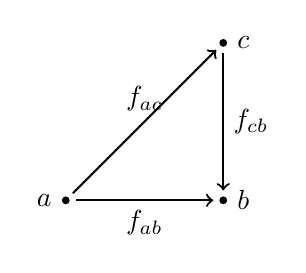
\begin{tikzpicture}[ele/.style={fill=black,circle,minimum
        width=.8pt,inner sep=1pt},every fit/.style={ellipse,draw,inner
        sep=-2pt}]
    
    \node[ele,label=left:$a$] (a) at (1,1) {};    
    \node[ele,label=right:$b$] (b) at (3,1) {};    
    \node[ele,label=right:$c$] (c) at (3,3) {};    
    
    \draw[->,thick,shorten <=2pt,shorten >=2pt] (a) to
    node[pos=0.5,above]{$f_{ac}$} (c);
    \draw[->,thick,shorten <=2pt,shorten >=2pt] (c) to
    node[pos=0.5,right]{$f_{cb}$} (b);
    \draw[->,thick,shorten <=2pt,shorten >=2pt] (a) to
    node[pos=0.5,below]{$f_{ab}$} (b);
  \end{tikzpicture}
  \caption{Commutative diagram for composition $f_{ab} = f_{cb} \circ f_{ac}$}
  \label{fig:composition}
\end{figure}
\end{example}


\begin{remark}[Class of Morphisms]
  \label{rem:morphclass}
  The \mynameref{def:class} of \mynameref{def:morphism}s will be marked as 
  $\cathom{C}$ (see \cref{fig:class_of_morphisms})
\end{remark}

\begin{figure}
  \centering
  \begin{tikzpicture}[ele/.style={fill=black,circle,minimum
        width=.8pt,inner sep=1pt},every fit/.style={ellipse,draw,inner
        sep=-2pt}]

    % the texts
    \node at (0,4) {$\cat{C}$};
    
    \node[ele,label=left:$a$] (a) at (0,2) {};    
    \node[ele,label=left:$b$] (b) at (0,1) {};    
    \node[ele,label=right:$c$] (c) at (2,2) {};
    \node[ele,label=right:$d$] (d) at (2,1) {};
    
    \node[draw,fit= (a) (b) (c) (d),minimum width=4cm, minimum
      height=4cm] {}  ;
    \draw[->,thick,shorten <=2pt,shorten >=2pt] (a) to
    node[pos=0.5,above]{$f$} (c); 
    \draw[->,thick,shorten <=2pt,shorten >=2pt] (b) to
    node[pos=0.5,left]{$g$} (a); 
    \draw[->,thick,shorten <=2pt,shorten >=2pt] (b) to
    node[pos=0.5,right]{$h$} (c); 


  \end{tikzpicture}
  \caption{Class of morphisms $\cathom{C}=\{f,g,h\}$, where $h = f
    \circ g$}
  \label{fig:class_of_morphisms}
\end{figure}


\begin{definition}[Monomorphism]
  \label{def:monomorphism}
  If $\forall g_1, g_2$ the equation 
  \[
  f \circ g_1 = f \circ g_2
  \]
  leads to 
  \[
  g_1 = g_2
  \]
  then $f$ is called \textit{monomorphism} (see
  \cref{fig:monomorphism}). The monomorphism between 
  $a$ and $b$ is denoted as $f: a \hookrightarrow b$ (see also
  \mynameref{def:injection} or ``one-to-one'' functions). 
  \index{``one-to-one'' function}

\begin{figure}[H]
  \centering
  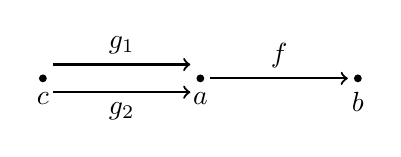
\begin{tikzpicture}[ele/.style={fill=black,circle,minimum
        width=.8pt,inner sep=1pt},every fit/.style={ellipse,draw,inner
        sep=-2pt}]

    \node[ele,label=below:$c$] (c) at (0,0) {};
    \node[ele,label=below:$a$] (a) at (2,0) {};    
    \node[ele,label=below:$b$] (b) at (4,0) {};    
    \draw[->,thick,shorten <=2pt,shorten >=2pt] (a) to
    node[pos=0.5,above]{$f$} (b); 
    \draw[->,thick,shorten <=2pt,shorten >=2pt] ([yshift=5pt] c.east) to         
         node[pos=0.5,above]{$g_1$} ([yshift=5pt] a.west); 
    \draw[->,thick,shorten <=2pt,shorten >=2pt] ([yshift=-5pt]c.east) to
         node[pos=0.5,below]{$g_2$} ([yshift=-5pt]a.west); 


  \end{tikzpicture}
  \caption{Monomorphism: $f \circ g_1 = f \circ g_2$ leads to $g_1 = g_2$}
  \label{fig:monomorphism}
\end{figure}


\end{definition}

\begin{definition}[Epimorphism]
  \label{def:epimorphism}
  If $\forall g_1, g_2$ the equation (see \cref{fig:epimorphism})
  \[
  g_1 \circ f = g_2 \circ f
  \]
  leads to 
  \[
  g_1 = g_2
  \]
  then $f$ is called \textit{epimorphism} (see also
  \mynameref{def:surjection} or ``onto'' functions).
  \index{``onto'' function}
\begin{figure}[H]
  \centering
  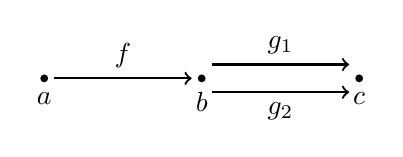
\begin{tikzpicture}[ele/.style={fill=black,circle,minimum
        width=.8pt,inner sep=1pt},every fit/.style={ellipse,draw,inner
        sep=-2pt}]

    \node[ele,label=below:$c$] (c) at (4,0) {};
    \node[ele,label=below:$a$] (a) at (0,0) {};    
    \node[ele,label=below:$b$] (b) at (2,0) {};    
    \draw[->,thick,shorten <=2pt,shorten >=2pt] (a) to
    node[pos=0.5,above]{$f$} (b); 
    \draw[->,thick,shorten <=2pt,shorten >=2pt] ([yshift=5pt]b.east) to
         node[pos=0.5,above]{$g_1$} ([yshift=5pt]c.west); 
    \draw[->,thick,shorten <=2pt,shorten >=2pt] ([yshift=-5pt]b.east) to
         node[pos=0.5,below]{$g_2$} ([yshift=-5pt]c.west); 


  \end{tikzpicture}
  \caption{Epimorphism: $g_1 \circ f = g_2 \circ f$ leads to $g_1 = g_2$}
  \label{fig:epimorphism}
\end{figure}

\end{definition}

\begin{definition}[Isomorphism]
\label{def:isomorphism} 
A \mynameref{def:morphism} $f: a \to b$ is called \textit{isomorphism} if
$\exists g: b \to a$ such that $f \circ g = \idm{a}$ 
and $g \circ f = \idm{b}$.  
If there is an isomorphism $f$ between objects $a$ and $b$
then it is denoted as $a \cong_f b$. 
\end{definition}

\begin{remark}[Isomorphism]
\label{rem:isomorphism}
There are can be many different \mynameref{def:isomorphism}s between 2
\mynameref{def:object}s. 

If there is an unique isomorphism between 2 objects then the objects
can be treated as the same object.
\end{remark}

\subsection{Category}

\begin{definition}[Category]
  \label{def:category}
  A category $\cat{C}$ consists of 
  \begin{itemize}
  \item \mynameref{def:class} of
    \mynameref{def:object}s $\catob{C}$
  \item \mynameref{def:class} of \mynameref{def:morphism}s $\cathom{C}$
    defined for $\catob{C}$, i.e. each morphism $f_{ab}$ from 
    $\cathom{C}$ has both source
    $a$ and target $b$ from $\catob{C}$
  \end{itemize}
  For any \mynameref{def:object} $a$ there should be unique
  \mynameref{def:id} $\idm{a}$. Any morphism should satisfy
  \mynameref{axm:composition} and \mynameref{axm:associativity} axioms
  (see example in \cref{fig:category}).    
\end{definition}

\begin{figure}
  \centering
  \begin{tikzpicture}[ele/.style={fill=black,circle,minimum
        width=.8pt,inner sep=1pt},every fit/.style={ellipse,draw,inner
        sep=-2pt}]

    % the texts
    \node at (0,4.5) {$\cat{C}$};
    
    \node[ele,label=left:$a$] (a) at (0,2) {};    
    \node[ele,label=left:$b$] (b) at (0,1) {};    
    \node[ele,label=right:$c$] (c) at (2,2) {};
    \node[ele,label=right:$d$] (d) at (2,1) {};
    
    \node[draw,fit= (a) (b) (c) (d),minimum width=5cm, minimum
      height=5cm] {}  ;
    \draw[->,thick,shorten <=2pt,shorten >=2pt] (a) to
    node[pos=0.5,above]{$f$} (c); 
    \draw[->,thick,shorten <=2pt,shorten >=2pt] (b) to
    node[pos=0.5,left]{$g$} (a); 
    \draw[->,thick,shorten <=2pt,shorten >=2pt] (b) to
    node[pos=0.5,right]{$h$} (c);

    \draw (a) to [out=45,in=135,looseness=20] node[above] {$\idm{a}$} (a);
    \draw (b) to [out=-45,in=-135,looseness=20] node[below] {$\idm{b}$} (b);
    \draw (c) to [out=45,in=135,looseness=20] node[above] {$\idm{c}$} (c);
    \draw (d) to [out=-45,in=-135,looseness=20] node[below] {$\idm{d}$} (d);

  \end{tikzpicture}
  \caption{Category $\cat{C}$. It consists of 4 objects
    $\catob{C} = \{a,b,c,d\}$ and 7 morphisms
    $\catob{C} = \{f,g,h = f \circ g, \idm{a}, \idm{b},
    \idm{c}, \idm{d}\}$}
  \label{fig:category}
\end{figure}

\begin{definition}[Set of morphisms]
\label{def:morphism_set}
  The set of morphisms between objects $a$ and $b$ in the category $\cat{C}$
  will be denoted as $\catmset[C]{a}{b}$. The set will be denoted
  as $\catmset{a}{b}$ if the exact category does not matter. 
\end{definition}

The \mynameref{def:category} can be considered as a way to represent a
structured data. \mynameref{def:morphism}s are the ones which form the
structure. 

\begin{definition}[Opposite category]
\label{def:op_category}
\index{Category!opposite}
\index{Category!dual}
If $\cat{C}$ is a \mynameref{def:category} then opposite (or dual) category
$\cat{C}^{op}$ is constructed in the following way: \mynameref{def:object}s
are the same, but the \mynameref{def:morphism}s are inverted i.e. 
if $f \in \cathom{C}$ and $\dom f = a, \cod f = b$, then the
corresponding morphism $f^{op} \in \cathom{C^{op}}$ has $\dom f^{op} =
b, \cod f^{op} = a$ (see \cref{fig:op_category})
\end{definition}

\begin{figure}
  \centering
  \begin{tikzpicture}[ele/.style={fill=black,circle,minimum
        width=.8pt,inner sep=1pt},every fit/.style={ellipse,draw,inner
        sep=-2pt}]

    % the texts
    \node at (0,4.5) {$\cat{C}$};
    
    \node[ele,label=left:$a$] (a) at (0,2) {};    
    \node[ele,label=left:$b$] (b) at (0,1) {};    
    \node[ele,label=right:$c$] (c) at (2,2) {};
    \node[ele,label=right:$d$] (d) at (2,1) {};
    
    \node[draw,fit= (a) (b) (c) (d),minimum width=5cm, minimum
      height=5cm] {}  ;
    \draw[->,thick,shorten <=2pt,shorten >=2pt] (c) to
    node[pos=0.5,above]{$f^{op}$} (a); 
    \draw[->,thick,shorten <=2pt,shorten >=2pt] (a) to
    node[pos=0.5,left]{$g^{op}$} (b); 
    \draw[->,thick,shorten <=2pt,shorten >=2pt] (c) to
    node[pos=0.5,right]{$h^{op}$} (b);

    \draw (a) to [out=45,in=135,looseness=20] node[above] {$\idm{a}$} (a);
    \draw (b) to [out=-45,in=-135,looseness=20] node[below] {$\idm{b}$} (b);
    \draw (c) to [out=45,in=135,looseness=20] node[above] {$\idm{c}$} (c);
    \draw (d) to [out=-45,in=-135,looseness=20] node[below] {$\idm{d}$} (d);

  \end{tikzpicture}
  \caption{Opposite category $C^{op}$ to the category from
    \cref{fig:category} . It consists of 4 objects
    $\catob{C^{op}} = \catob{C} = \{a,b,c,d\}$ and 7 morphisms
    $\cathom{C^{op}} = \{f^{op},g^{op},h^{op} = g^{op} \circ
    f^{op}, \idm{a}, \idm{b}, 
    \idm{c}, \idm{d}\}$}
  \label{fig:op_category}
\end{figure}

\begin{remark}{Composition on $C^{op}$}
\label{rem:op_composition}
\index{Composition!opposite category}
As you can see from \cref{fig:op_category} the
\mynameref{axm:composition} is reverted for
\mynameref{def:op_category}. If $f,g,h = f \circ g \in
\cathom{C}$ then $f \circ g$ translated into $g^{op} \circ
f^{op}$ in opposite category.
\end{remark}

\begin{definition}[Small category]
\label{def:small_category}
\index{Category!small}
A category $\cat{C}$ is called \textit{small} if both $\catob{C}$ and
$\cathom{C}$ are \nameref{def:set}s
\end{definition}

\begin{definition}[Locally small category]
\label{def:localy_small_category}
\index{Category!locally small}

A category $\cat{C}$ is called \textit{locally small} if 
$\cathom{C}$ is a \nameref{def:set}. The set is called \mynameref{def:homset}.
\end{definition}

\begin{definition}[Homset]
\label{def:homset}
The \textit{homset} is the \mynameref{def:set} of morphisms in a
\mynameref{def:localy_small_category}. 
\end{definition}


\begin{definition}[Large category]
\label{def:large_category}
\index{Category!large}
A category $\cat{C}$ is not \mynameref{def:small_category} then it is
called \textit{large}. The example of large category is
\mynameref{def:setcategory} 
\end{definition}

\begin{definition}[Empty category]
\label{def:empty_category}
The category that does not contain any \mynameref{def:object}s and as
result does not contain any \mynameref{def:morphism}s is called
\textit{Empty category} \cite{bib:stackexchange:empty_category}.
\end{definition}

\begin{definition}[Trivial category]
\label{def:trivial_category}
The category that contains only one \mynameref{def:object} and only
one \mynameref{def:morphism} (\mynameref{def:id})  is called
\textit{Trivial category}.
\end{definition}

There are several examples of categories below that will also be used
later:
\begin{itemize}
\item $\cat{Set}$ category example: see \cref{sec:setcategory_example}
\item Programming languages (Haskell, C\texttt{++}, Scala) examples: see
  \cref{sec:plcategory_example}
\item Quantum mechanics example: see \cref{sec:qmcategory_example}
\end{itemize}

\section{$\cat{Set}$ category example}
\label{sec:setcategory_example}
The category of sets is the most important example because it will
allow connect our usual knowledge about sets with the category theory. 

\begin{definition}[Set]
  \label{def:set}
  \textit{Set} is a collection of distinct objects. The objects are called as
  the elements of the set. 

  The set will be denoted by a capital letter in
  the book, for instance $A$. The elements of a set will be denoted by
  small letters: $a \in A$.
\end{definition}

\begin{definition}[Cartesian product]
  \label{def:cartesian_product}
  If $A$ and $B$ are two sets then we can define a new set $A \times B
  = \left\{(a,b)|a \in A, b \in B\right\}$ that is called as the
  \textit{cartesian product}.
\end{definition}

\begin{definition}[Binary relation]
  \label{def:binary_relation}
  If $A$ and $B$ are 2 \mynameref{def:set}s then a subset of the
  \mynameref{def:cartesian_product} $A \times B$ is
  called as \textit{binary relation} $R$ between the 2 sets, i.e. $R
  \subset A \times B$. 
\end{definition}

\begin{definition}[Function]
  \label{def:function}
  \textit{Function} $f$ is a special type of \mynameref{def:binary_relation}. I.e.
  if $A$ and $B$ are 2 \mynameref{def:set}s then a subset of $A \times B$ is
  called function $f$ between the 2 sets if $\forall a \in A \, \exists!
  b \in B$ such that $(a,b) \in f$. In other words function definition
  does not allow ``multi value''.
\end{definition}

\begin{definition}[$\cat{Set}$ category]
  \label{def:setcategory}
  \index{Object!$\cat{Set}$ category}
  \index{Morphism!$\cat{Set}$ category}
  \index{Category!$\cat{Set}$}
  In the \textit{Set category} we consider a
  \mynameref{def:set} of 
  \mynameref{def:set}s where 
  \mynameref{def:object}s are the \mynameref{def:set}s and
  \mynameref{def:morphism}s are \mynameref{def:function}s between the
  sets.The \mynameref{def:id} is the trivial function such that $\forall x \in
  X: \idm{X}(x) = x$.
\end{definition}

\begin{remark}[$\cat{Set}$ category]
  In general case when we say $\cat{Set}$ category we assume the set
  of all sets. But the result is inconsistent because famous Russell's
  paradox \cite{wiki:russell_paradox} can be applied. To avoid such
  situations we consider a limitation that is applied on our
  construction, for instance 
  ZFC \cite{wiki:zfc}. If we apply the limitation we have that set of
  all sets is not a set itself and as result the  $\cat{Set}$
  category is a \mynameref{def:large_category}
  \index{Category!large}
\end{remark}

\begin{remark}[Set vs Category]
  \label{rem:set_vs_category}
  There is an interesting relation between sets and categories. In both
  we consider objects(sets) and relations between
  them(morphisms/functions). 

  In the set theory we can get info about functions by looking inside
  the objects(sets) aka use ``microscope'' \cite{bib:milewski2018category} 

  Contrary in the category theory we initially don't have any info about object
  internal structure but can get it using the relation between the
  objects i.e. using \mynameref{def:morphism}s. In other words we can use
  ``telescope'' \cite{bib:milewski2018category}  there.
\end{remark}

\begin{definition}[Categorical approach]
\label{def:categorical_approach}
The description of a system (object) via its relations with other
systems (objects) will be called as  \textit{categorical approach} in
the book. This description is an alternative one to an ordinary system
description via its internal structure.
\end{definition}

\begin{definition}[Singleton]
\label{def:singleton_set} 
The \textit{singleton} is a \mynameref{def:set} with only one element.
\end{definition}

\begin{example}[Domain]
  \label{ex:domain_set}
  Given a function $f: X \to Y$, the set $X$ is the domain. I.e. $\dom
  f = X$
\end{example}

\begin{example}[Codomain]
  \label{ex:codomain_set}
  Given a function $f: X \to Y$, the set $Y$ is the codomain. I.e.
  $\cod f = Y$
\end{example}

\begin{definition}[Image]
\label{def:function_image} 
The \textit{image} of a function $f: X \to Y$ is a subset of
\mynameref{def:codomain} $Y$ such that for every element in the subset
there is an element in \mynameref{def:domain} $X$ that maps into the
subset:
\[
\Ima{f} = \{y \in Y| y = f(x) \mbox{ for some } x \in X\}
\]
\end{definition}


\begin{definition}[Surjection]
  \label{def:surjection}
  \index{``onto'' function}
  The function $f: X \rightarrow Y$ is \textit{surjective} (or ``onto'') if
  $\forall y \in Y$, $\exists x \in X$ such that
  $f\left(x\right) = y$ (see \cref{fig:surjection,fig:bijection}).
\end{definition}

\begin{example}[Surjection]
An example of a surjective function is shown in \cref{fig:surjection}.
Note that the function in the figure is not an
\mynameref{def:injection}. You can find an example of a function that
is \mynameref{def:surjection} as well as \mynameref{def:injection} (aka
\mynameref{def:bijection}) in \cref{fig:bijection}.
\begin{figure}[H]
  \centering
  \begin{tikzpicture}[ele/.style={fill=black,circle,minimum
        width=.8pt,inner sep=1pt},every fit/.style={ellipse,draw,inner
        sep=-2pt}]

    % the texts
    \node at (0,5) {$X$};
    \node at (4,5) {$Y$};
    
    \node[ele,label=left:$x_1$] (x1) at (0,4) {};    
    \node[ele,label=left:$x_2$] (x2) at (0,3) {};    
    \node[ele,label=left:$x_3$] (x3) at (0,2) {};
    \node[ele,label=left:$x_4$] (x4) at (0,1) {};

    \node[ele,,label=right:$y_1$] (y1) at (4,4) {};
    \node[ele,,label=right:$y_2$] (y2) at (4,3) {};
    \node[ele,,label=right:$y_3$] (y3) at (4,2) {};

    \node[draw,fit= (x1) (x2) (x3) (x4),minimum width=2cm] {} ;
    \node[draw,fit= (y1) (y2) (y3),minimum width=2cm] {} ;  
    \draw[->,thick,shorten <=2pt,shorten >=2pt] (x1) -- (y2);
    \draw[->,thick,shorten <=2pt,shorten >=2] (x2) -- (y1);
    \draw[->,thick,shorten <=2pt,shorten >=2] (x3) -- (y3);
    \draw[->,thick,shorten <=2pt,shorten >=2] (x4) -- (y3);
  \end{tikzpicture}
  \caption{A surjective (non-injective) function from domain $X$ to
    codomain $Y$ }
  \label{fig:surjection}
\end{figure}
\end{example}

\begin{remark}[Surjection vs Epimorphism]
  \label{rem:surjection_epimorphism}
  \mynameref{def:surjection} and \mynameref{def:epimorphism} are
  related each other. Consider a non-surjective function $f: X
  \rightarrow Y' \subset Y$ (see \cref{fig:surjection_epimorphism}). One can
  conclude that there is not an \mynameref{def:epimorphism} because  
  $\exists g_1: Y' \to Y'$ and  $g_2 : Y \to Y$ such
  that $g_1 \ne g_2$ because they operates on different
  \mynameref{def:domain}s but from other hand $g_1(y) = g_2(y),
  \forall y \in Y'$. For
  instance we can choose $g_1 = \idm{Y'}, g_2=\idm{Y}$. As
  soon as $Y'$ is \mynameref{def:codomain} of $f$ we always have
  $g_1(f(x)) = g_2(f(x))$, $\forall x \in X$. I.e. 
  \[
  g_1 \circ f = g_2 \circ f,
  \]
  but $g_1 \ne g_2$. As result one can say that a
  \mynameref{def:surjection} is an 
  \mynameref{def:epimorphism} in the $\cat{Set}$ category. Moreover
  there is a proof 
  \cite{bib:proofwiki:Surjection_iff_Epimorphism_in_Category_of_Sets}
  of that fact.

\end{remark}


% https://tex.stackexchange.com/questions/19987/
% drawing-a-bijective-map-with-tikz 
\begin{figure}
  \centering
  \begin{tikzpicture}[ele/.style={fill=black,circle,minimum
        width=.8pt,inner sep=1pt},every fit/.style={ellipse,draw,inner
        sep=-2pt}]

    % the texts
    \node at (0,5) {$X$};
    \node at (4,5) {$Y$};
    \node at (5.5,3.5) {$Y'$};
    
    \node[ele,label=left:$x_1$] (x1) at (0,4) {};    
    \node[ele,label=left:$x_2$] (x2) at (0,3) {};    
    \node[ele,label=left:$x_3$] (x3) at (0,2) {};
    \node[ele,label=left:$x_4$] (x4) at (0,1) {};

    \node[ele,,label=right:$y_1$] (y1) at (4,4) {};
    \node[ele,,label=right:$y_2$] (y2) at (4,3) {};
    \node[ele,,label=right:$y_3$] (y3) at (4,2) {};
    \node[ele,,label=right:$y_4$] (y4) at (4,1) {};
    
    \node[draw,fit= (x1) (x2) (x3) (x4),minimum width=2cm] {} ;
    \node[draw,fit= (y1) (y2) (y3) (y4),minimum width=2cm] {} ;
    \node[draw,fit= (y1) (y2) (y3),minimum width=2cm] {} ;
    \draw[->,thick,shorten <=2pt,shorten >=2pt] (x1) -- (y2);
    \draw[->,thick,shorten <=2pt,shorten >=2] (x2) -- (y1);
    \draw[->,thick,shorten <=2pt,shorten >=2] (x3) -- (y3);

  \end{tikzpicture}
  \caption{A non-surjective function $f$ from domain $X$ to
    codomain $Y' \subset Y$.
    $\exists g_1: Y' \rightarrow Y', g_2: Y \rightarrow Y$ such that
    $g_1(y) = g_2(y), \forall y \in Y'$, but as soon as $Y' 
    \ne Y$ we have $g_1 \ne g_2$. Using the fact that $Y'$ is codomain
    of $f$ we got $g_1 \circ f = g_2 \circ f$.
    I.e. the function $f$ is not epimorphism. }
  \label{fig:surjection_epimorphism}
\end{figure}


\begin{definition}[Injection]
  \label{def:injection}
  \index{``one-to-one'' function}
  The function $f: X \rightarrow Y$ is injective (or ``one-to-one'' function) if
  $\forall x_1, x_2 \in X$, such that $x_1 \ne x_2$ then
  $f\left(x_1\right) \ne f\left(x_2\right)$ (see
  \cref{fig:injection,fig:bijection}).  
\end{definition}

\begin{example}[Injection]
% https://tex.stackexchange.com/questions/19987/
% drawing-a-bijective-map-with-tikz 
An example of an injective function is shown in \cref{fig:injection}.
Note that the function in the figure is not a
\mynameref{def:surjection}. You can find an example of a function that
is \mynameref{def:surjection} as well as \mynameref{def:injection} (aka
\mynameref{def:bijection}) in \cref{fig:bijection}.
\begin{figure}[H]
  \centering
  \begin{tikzpicture}[ele/.style={fill=black,circle,minimum
        width=.8pt,inner sep=1pt},every fit/.style={ellipse,draw,inner
        sep=-2pt}]

    % the texts
    \node at (0,5) {$X$};
    \node at (4,5) {$Y$};
    
    \node[ele,label=left:$x_1$] (x1) at (0,4) {};    
    \node[ele,label=left:$x_2$] (x2) at (0,3) {};    
    \node[ele,label=left:$x_3$] (x3) at (0,2) {};
    \node[ele,label=left:$x_4$] (x4) at (0,1) {};

    \node[ele,,label=right:$y_1$] (y1) at (4,4) {};
    \node[ele,,label=right:$y_2$] (y2) at (4,3) {};
    \node[ele,,label=right:$y_3$] (y3) at (4,2) {};
    \node[ele,,label=right:$y_4$] (y4) at (4,1) {};

    \node[draw,fit= (x1) (x2) (x3) (x4),minimum width=2cm] {} ;
    \node[draw,fit= (y1) (y2) (y3) (y4),minimum width=2cm] {} ;  
    \draw[->,thick,shorten <=2pt,shorten >=2pt] (x1) -- (y2);
    \draw[->,thick,shorten <=2pt,shorten >=2] (x2) -- (y1);
    \draw[->,thick,shorten <=2pt,shorten >=2] (x3) -- (y3);
  \end{tikzpicture}
  \caption{A injective (non-surjective) function from domain $X$ to
    codomain $Y$ }
  \label{fig:injection}
\end{figure}
\end{example}

\begin{remark}[Injection vs Monomorphism]
  \label{rem:injection_monomorphism}
  \mynameref{def:injection} and \mynameref{def:monomorphism} are
  related each other. Consider a non-injective function $f: X
  \rightarrow Y$ (see \cref{fig:injection_monomorphism}). One can
  conclude that it is not a \mynameref{def:monomorphism} because
  $\exists g_1, g_2$ such 
  that $g_1 \ne g_2$ and $f(g_1(a_1)) = y_3 = f(g_2(b_1))$. As result
  one can say that an \mynameref{def:injection} is a
  \mynameref{def:monomorphism} in the $\cat{Set}$ category. Moreover there
  is a proof
  \cite{bib:proofwiki:Injection_iff_Monomorphism_in_Category_of_Sets} 
  of that fact.
\end{remark}

\begin{figure}
  \centering
  \begin{tikzpicture}[ele/.style={fill=black,circle,minimum
        width=.8pt,inner sep=1pt},every fit/.style={ellipse,draw,inner
        sep=-2pt}]

    % the texts
    \node at (0,5) {$A$};
    \node at (0,0) {$B$};
    \node at (4,5) {$X$};
    \node at (8,5) {$Y$};

    \node[ele,label=left:$a_1$] (a1) at (0,4) {};
    \node[ele,label=left:$a_2$] (a2) at (0,3) {};    

    \node[ele,label=left:$b_1$] (b1) at (0,2) {};    
    \node[ele,label=left:$b_2$] (b2) at (0,1) {};    

    
    \node[ele,label=left:$x_1$] (x1) at (4,4) {};    
    \node[ele,label=left:$x_2$] (x2) at (4,3) {};    
    \node[ele,label=left:$x_3$] (x3) at (4,2) {};
    \node[ele,label=left:$x_4$] (x4) at (4,1) {};

    \node[ele,,label=right:$y_1$] (y1) at (8,4) {};
    \node[ele,,label=right:$y_2$] (y2) at (8,3) {};
    \node[ele,,label=right:$y_3$] (y3) at (8,2) {};
    \node[draw,fit= (a1) (a2),minimum width=2cm] {} ;
    \node[draw,fit= (b1) (b2),minimum width=2cm] {} ;

    \node[draw,fit= (x1) (x2) (x3) (x4),minimum width=2cm] {} ;
    \node[draw,fit= (y1) (y2) (y3),minimum width=2cm] {} ;  

    \draw[->,thick,shorten <=2pt,shorten >=2pt] (x1) -- (y2);
    \draw[->,thick,shorten <=2pt,shorten >=2] (x2) -- (y1);
    \draw[->,thick,shorten <=2pt,shorten >=2] (x3) -- (y3);
    \draw[->,thick,shorten <=2pt,shorten >=2] (x4) -- (y3);

    \draw[->,thick,shorten <=2pt,shorten >=2] (a1) -- (x3);
    \draw[->,thick,shorten <=2pt,shorten >=2] (a2) -- (x3);

    \draw[->,thick,shorten <=2pt,shorten >=2] (b1) -- (x4);
    \draw[->,thick,shorten <=2pt,shorten >=2] (b2) -- (x4);

  \end{tikzpicture}
  \caption{A non-injective function $f$ from domain $X$ to
    codomain $Y$. $\exists g_1: A \rightarrow X, g_2: B
    \rightarrow X$ such that $g_1 \ne g_2$ (as soon as the functions
    operate on different domains) but $f
    \circ g_1 = f \circ g_2$. I.e. the function $f$ is not a monomorphism. }
  \label{fig:injection_monomorphism}
\end{figure}


\begin{figure}
  \centering
  \begin{tikzpicture}[ele/.style={fill=black,circle,minimum
        width=.8pt,inner sep=1pt},every fit/.style={ellipse,draw,inner
        sep=-2pt}]
    % the texts
    \node at (0,5) {$X$};
    \node at (4,5) {$Y$};
    
    \node[ele,label=left:$x_1$] (x1) at (0,4) {};    
    \node[ele,label=left:$x_2$] (x2) at (0,3) {};    
    \node[ele,label=left:$x_3$] (x3) at (0,2) {};
    \node[ele,label=left:$x_4$] (x4) at (0,1) {};

    \node[ele,,label=right:$y_1$] (y1) at (4,4) {};
    \node[ele,,label=right:$y_2$] (y2) at (4,3) {};
    \node[ele,,label=right:$y_3$] (y3) at (4,2) {};
    \node[ele,,label=right:$y_4$] (y4) at (4,1) {};

    \node[draw,fit= (x1) (x2) (x3) (x4),minimum width=2cm] {} ;
    \node[draw,fit= (y1) (y2) (y3) (y4),minimum width=2cm] {} ;  
    \draw[->,thick,shorten <=2pt,shorten >=2pt] (x1) -- (y4);
    \draw[->,thick,shorten <=2pt,shorten >=2] (x2) -- (y2);
    \draw[->,thick,shorten <=2pt,shorten >=2] (x3) -- (y1);
    \draw[->,thick,shorten <=2pt,shorten >=2] (x4) -- (y3);
  \end{tikzpicture}
  \caption{An injective and surjective function (bijection)}
  \label{fig:bijection}
\end{figure}

\begin{definition}[Bijection]
  \label{def:bijection}
  \index{``one-to-one'' correspondence}
  The function $f: X \rightarrow Y$ is bijective (or ``one-to-one''
  correspondence) if it is an \mynameref{def:injection} and a
  \mynameref{def:surjection} (see \cref{fig:bijection}). 
\end{definition}

There is a question what is the categorical analog of a single
\mynameref{def:set}. Main characteristic of a category is a structure
but the \mynameref{def:set} by definition does not have a structure.
Which category 
does not have any structure? The answer is
the \mynameref{def:discrete_category}. 

\begin{definition}[Discrete category]
  \label{def:discrete_category}
  Discrete category is a \mynameref{def:category} where
  \mynameref{def:morphism}s are only \mynameref{def:id}s.
\end{definition}
  
\section{Programming languages examples}
\label{sec:plcategory_example}
Functions are the most important
constructions in programming languages. They allow to convert elements 
\footnote{
We consider variables as the elements in Scala, C\texttt{++} and 
CAF (Constant applicative form) as the elements in Haskell
} of one type into elements of another one. 

\begin{definition}[Pure function]
\label{def:pure_function}
The function is pure if it's execution give the same results
independently from the environment. 
\end{definition}

Categorical view to programming languages assumes types as
\mynameref{def:object}s and functions as
\mynameref{def:morphism}s. The critical requirements for such
consideration is that the functions have to be
\mynameref{def:pure_function}s (without side effects). This requirement
mainly is satisfied by functional languages such as Haskell and Scala.

From other side the functional languages use lazy evaluation to
improve their performance. The laziness can also make category theory
axiom invalid (see \mynameref{rem:hask_lazy_eval} below). 

%http://math.andrej.com/2016/08/06/hask-is-not-a-category/
\begin{remark}[Haskell lazy evaluation]
  \label{rem:hask_lazy_eval}
  Each Haskell type has a special value $\bot$. The fact that the
  value and the lazy evaluations are parts of the language, make several
  category law invalid, for instance 
  \mynameref{def:id} behaviour become invalid in specific cases:

  The following code
  \begin{minted}{haskell}
    seq undefined True
  \end{minted}
  produces \textit{undefined}
  But the following
  \begin{minted}{haskell}
    seq (id.undefined) True
    seq (undefined.id) True
  \end{minted}
  produces \textit{True} in both cases.
  As result we have
  \footnote{we cannot compare functions in Haskell, but if we
  could we can get it}
  \begin{minted}{haskell}
    id . undefined /= undefined
    undefined . id /= undefined,
  \end{minted}
  i.e. \eqref{eq:leftid} and
  \eqref{eq:rightid} are not satisfied.  
\end{remark}

Strictly speaking neither Haskell (pure functional language) nor C\texttt{++}
can be considered as a category in general. For the first approximation
a functional language (Haskell, Scala) can be considered as a
category if we avoid to use functions with side effects (mainly for
Scala) and use strict, not lazy, evaluations (for both Haskell and
Scala). Take the fact into consideration and define categories for 3
languages 

\begin{definition}[$\cat{Hask}$ category]
\label{def:haskcategory}
The objects in the $\cat{Hask}$ category are Haskell types and
morphisms are functions
\end{definition}

\begin{definition}[$\cat{Scala}$ category]
\label{def:scalacategory}
The objects in the $\cat{Scala}$ category are Scala types and
morphisms are functions. We don't define functions that have a state
in the category. I.e. the functions are \mynameref{def:pure_function}s. 
\end{definition}

\begin{definition}[$\cat{C\texttt{++}}$ category]
\label{def:cppcategory}
The objects in the $\cat{C\texttt{++}}$ category are C\texttt{++}
types and morphisms are functions. We don't define functions that have
a state in the category. I.e. the functions are
\mynameref{def:pure_function}s.  
\end{definition}


In any case we can construct a simple toy category that can be easy
implemented in any language. Particularly we will look into category
with 3 \mynameref{def:object}s that are types: \textbf{Int}, \textbf{Bool},
\textbf{String}. There are also several \mynameref{def:morphism}s
(functions) between them (see \cref{fig:pl_example}).    

\begin{figure}
  \centering
  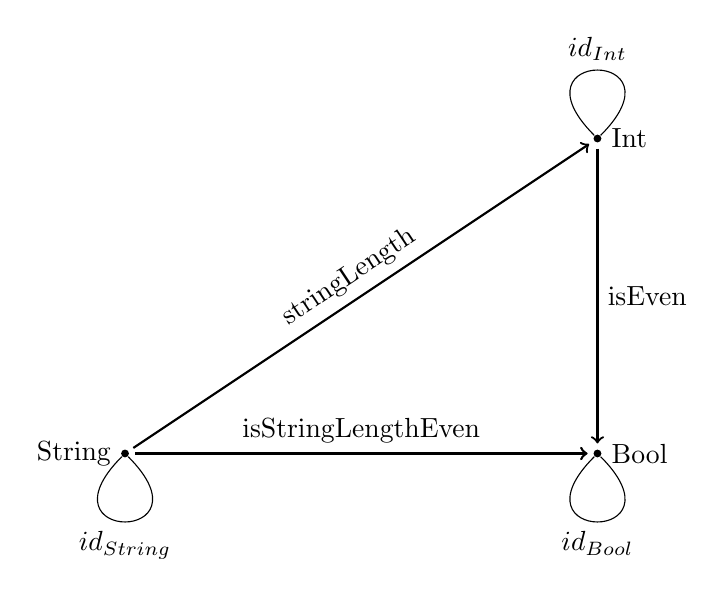
\begin{tikzpicture}[ele/.style={fill=black,circle,minimum
        width=.8pt,inner sep=1pt},every fit/.style={ellipse,draw,inner
        sep=-2pt}]
    % the texts    
    \node[ele,label=right:Int] (int) at (6,4) {};    
    \node[ele,label=right:Bool] (bool) at (6,0) {};    
    \node[ele,label=left:String] (string) at (0,0) {};

    \draw[->,thick,shorten <=2pt,shorten >=2pt] (int) to
    node[right]{isEven} (bool); 
    \draw[->,thick,shorten <=2pt,shorten >=2] (string) to
    node[pos=0.5,sloped,above]{stringLength} (int); 
    \draw[->,thick,shorten <=2pt,shorten >=2] (string) to
    node[pos=0.5,sloped,above]{isStringLengthEven} (bool); 
    \draw[->,thick,shorten <=2pt,shorten >=2] (string) -- (bool);
    \draw (int) to [out=45,in=135,looseness=50] node[above]
          {$id_{Int}$} (int); 
    \draw (string) to [out=-45,in=-135,looseness=50] node[below]
          {$id_{String}$} (string); 
    \draw (bool) to [out=-45,in=-135,looseness=50] node[below]
          {$id_{Bool}$} (bool); 

  \end{tikzpicture}
  \caption{Programming language category example. Objects are types: Int,
    Bool, String. Morphisms are several functions}
  \label{fig:pl_example}
\end{figure}


\subsection{$\cat{Hask}$ toy category}
\begin{example}[$\cat{Hask}$ toy category]
  \label{ex:haskcategory}
  \index{Object!$\cat{Hask}$ example}
  \index{Morphism!$\cat{Hask}$ example}
  Types in Haskell are considered as \mynameref{def:object}s.
  Functions are considered as \mynameref{def:morphism}s.
  We are going to implement \mynameref{def:category} from
  \cref{fig:pl_example}.

  The function \textbf{isEven}
  converts \textbf{Int} type 
  into \textbf{Bool}.
  \begin{minted}{haskell}
    isEven :: Int -> Bool
    isEven x = x `mod` 2 == 0
  \end{minted}

  There is also \mynameref{def:id} that is defined as follows
  \begin{minted}{haskell}
    id :: a -> a
    id x = x
  \end{minted}

  If we have an additional function
  \begin{minted}{haskell}
    stringLength :: String -> Int
    stringLength x = length x
  \end{minted}
  then we can create a \mynameref{axm:composition}
  \begin{minted}{haskell}
    isStringLengthEven :: String -> Bool
    isStringLengthEven = isEven . stringLength
  \end{minted}

  %% If we consider pure (without effects) functions then
  %% \mynameref{axm:associativity} is also satisfied.
\end{example}

\subsection{$\cat{Scala}$ toy category}
\begin{example}[$\cat{Scala}$ toy category]
  \label{ex:scalacategory}
  \index{Object!$\cat{Scala}$ example}
  \index{Morphism!$\cat{Scala}$ example}

  We will use the same trick as in \mynameref{ex:haskcategory} and
  will assume 
  types in Scala as \mynameref{def:object}s, 
  functions as \mynameref{def:morphism}s.
  We also are going to implement
  \mynameref{def:category} from \cref{fig:pl_example}.

  \begin{minted}{scala}
    object Category {
      def id[A]: A => A = a => a
      def compose[A, B, C](g: B => C, f: A => B): 
          A => C = g compose f 
      
      val isEven = (i: Int) => i % 2  == 0
      val stringLength = (s: String) => s.length
      val isStringLengthEven = (s: String) => 
          compose(isEven, stringLength)(s)
    }
  \end{minted}

  The usage example is below
  \begin{minted}{scala}
    
    class CategorySpec extends Properties("Category") {
      import Category._
      import Prop.forAll
      
      property("composition") = forAll { (s: String) =>
        isStringLengthEven(s)  == isEven(stringLength(s))
      }
      
      property("right id") = forAll { (i: Int) =>
        isEven(i)  == compose(isEven, id[Int])(i)
      }
      
      property("left id") = forAll { (i: Int) =>
        isEven(i)  == compose(id[Boolean], isEven)(i)
      }
    }
  \end{minted}
\end{example}

\subsection{$\cat{C\texttt{++}}$ toy category}
\begin{example}[$\cat{C\texttt{++}}$ toy category]
  \label{ex:cppcategory}
  \index{Object!$\cat{C\texttt{++}}$ example}
  \index{Morphism!$\cat{C\texttt{++}}$ example}
  We will use the same trick as in \mynameref{ex:haskcategory} and
  will assume 
  types in C\texttt{++} as \mynameref{def:object}s, 
  functions as \mynameref{def:morphism}s.
  We also are going to implement
  \mynameref{def:category} from \cref{fig:pl_example}.


  We  also define 2 functions:
  \begin{minted}{c++}
    auto isEven = [](int x) { 
      return x % 2 == 0; 
    };

    auto stringLength = [](std::string s) { 
      return static_cast<int>(s.size()); 
    };
  \end{minted}

  Composition can be defined as follows:
  \begin{minted}{c++}
    // h = g . f
    template <typename A, typename B> 
    auto compose(A g, B f) {
      auto h = [f, g](auto a) {
        auto b = f(a);
        auto c = g(b);
        return c;
      };
      return h;
    };
  \end{minted}

  The \mynameref{def:id}:
  \begin{minted}{c++}
    auto id = [](auto x) { return x; };
  \end{minted}

  The usage examples are the following:
  \begin{minted}{c++}
    auto isStringLengthEven = compose<>(isEven, stringLength);

    auto isStringLengthEvenL = compose<>(id, isStringLengthEven);

    auto isStringLengthEvenR = compose<>(isStringLengthEven, id);  
  \end{minted}

  Such construction will always provides us the category as soon as we
  use pure function (functions without effects).
\end{example}


\section{Quantum mechanics examples}
\label{sec:qmcategory_example}
The most critical property of quantum system is the superposition
principle. The \mynameref{def:setcategory} cannot be used for it
because it does not satisfy the principle. but a simple modification
of the $\cat{Set}$ category does. 
\begin{definition}[$\cat{Rel}$ category]
  \label{def:relcategory}
  \index{Object!$\cat{Rel}$ category}
  \index{Morphism!$\cat{Rel}$ category}
  We will consider a set of sets (same as \mynameref{def:setcategory})
  i.e. \mynameref{def:set}s as \mynameref{def:object}s. Instead of
  \mynameref{def:function}s we will use \mynameref{def:binary_relation}s as
  \mynameref{def:morphism}s. 

  The $\cat{Rel}$ category is similar to the finite dimensional
  Hilber space especially because it assumes some kind of superposition.
  Really consider $\cat{Rel}$ - the $\cat{Rel}$ category. $X, Y \in
  \catob{Rel}$ - 2 sets which consists of different elements. Let $f: X
  \to X$ - \mynameref{def:morphism}. Each element $x \in X$ is
  mapped to a subset $Y' \subset Y$. The $Y'$ can be
  \mynameref{def:singleton_set}  (in this case no differences with
  \mynameref{def:setcategory}) but there can be a situation when $Y'$
  consists of several elements. In the case we will get some kind of
  superposition that is analogiest to quantum systems.
\end{definition}

In the quantum mechanics we say about Hilber spaces.
\begin{definition}[Hilbert space]
  \label{def:hilbert_space} The Hilbert space is a complex vector space
  with an inner product as a complex number ($\mathbb{C}$).

  Later we will consider only finite dimensional Hilber spaces.
  We will denote a Hilbert space of dimensional $n$ as
  $\mathcal{H}_n$. Obviously $\mathcal{H}_1 = \mathbb{C}$.
\end{definition}

\begin{definition}[Dual space]
\label{def:dual_space}
Each Hilber space $\mathcal{H}$ has an associated with it dual space
$\mathcal{H}^\ast$ that consists of linear functionals  
\end{definition}

\begin{example}[Dirac notation]
\label{ex:dirac_notation}
Consider a ket-vector $\ket{\psi} \in \mathcal{H}$. Then the
corresponding vector from \mynameref{def:dual_space} is called
bra-vector $\bra{\psi} \in \mathcal{H}^\ast$. From the definition of
dual space the bra-vector is a linear functional i.e. 
\[
\bra{\psi} : \mathcal{H} \to \mathbb{C},
\]
$\forall \ket{\phi} \in \mathcal{H}$ we have 
\(
\bra{\psi}\left(\ket{\phi}\right) = \left(\ket{\psi}, \ket{\phi}\right)
\) - inner product that is often written as $\bra{\psi}\ket{\phi}$.
\end{example}


The
transformation between 2 \mynameref{def:hilbert_space}s that preserves
the structure is called 
linear map or linear transformations.
\begin{definition}[Linear map]
\label{def:linear_map}
The linear map between2 \mynameref{def:hilbert_space}s $\mathcal{A}$
and $\mathcal{B}$ is a mapping $f: \mathcal{A} \to \mathcal{B}$ that
preserves additions  
\[
f(a_1 + a_2) = f(a_1) + f(a_2),
\]
and scalar multiplications:
\[
f(c \cdot a) = c \cdot f(a)
\]
where $a,a_{1,2} \in \mathcal{A}$ and $f(a), f(a_{1,2}) \in \mathcal{B}$.
\end{definition}

\begin{remark}[Linear map]
\label{rem:linear_map} 
Note that \mynameref{def:linear_map} does not preserve inner product.
TBD (verify the statement ???)
\end{remark}

If we want to combine 2 Hilbert spaces into one we use a notion of
direct sum.
\begin{definition}[Direct sum of Hilber spaces]
  \label{def:fdhilb_direct_sum}
  Let $\mathcal{A}, \mathcal{B}$ are 2 Hilber spaces. The
  direct sum $\mathcal{A} \oplus \mathcal{B}$ is defined as follows
  \[
  \mathcal{A} \oplus \mathcal{B} = \{a \oplus b | a \in \mathcal{A}, b
  \in \mathcal{B}\}.
  \]
  The inner product is defined as follows
  \[
  \bra{a_1 \oplus b_1}\ket{a_2 \oplus b_2} =
  \bra{a_1}\ket{a_2} + \bra{b_1}\ket{b_2}.
  \]
\end{definition}

\begin{definition}[$\cat{FdHilb}$ category]
  \label{def:fdhilbcategory}
  \index{Object!$\cat{FdHilb}$ category}
  \index{Morphism!$\cat{FdHilb}$ category}

  Most common case in quantum mechanics is the case of quantum states
  in the finite dimensional Hilbert space. We can consider the set of
  all finite dimensional Hilbert spaces as a category. The
  \mynameref{def:object}s in the category are finite dimensional
  \mynameref{def:hilbert_space}s and \mynameref{def:morphism}s are
  \mynameref{def:linear_map}s. The category is denoted as
  $\cat{FdHilb}$. It is very similar to   \mynameref{def:relcategory}.
  The brief relation is   described in the
  \cref{tab:set_vs_rel_vs_fdhilb}.  
  \begin{table}
    \centering
    \caption{Relations between $\cat{Set}$, $\cat{Rel}$ and $\cat{FdHilb}$ categories}
    \label{tab:set_vs_rel_vs_fdhilb}
    \begin{adjustbox}{width=1\textwidth}
      \small
      \begin{tabular}{l|l|l|l}
        \toprule
        & $\cat{Set}$ & $\cat{Rel}$ & $\cat{FdHilb}$\\
        \midrule
        \mynameref{def:object} & \mynameref{def:set} &
        \mynameref{def:set} &
        finite dimensional \mynameref{def:hilbert_space}\\
        \mynameref{def:morphism} & \mynameref{def:function} &
          \mynameref{def:binary_relation} & 
          \mynameref{def:linear_map}\\
          \mynameref{def:initial_object} & empty set & empty set & trivial
          \mynameref{def:hilbert_space} of dimensional 0 \\
          \mynameref{def:terminal_object} & \mynameref{def:singleton_set} &
          \mynameref{def:singleton_set} & $\mathbb{C}$ \\
          \mynameref{def:product} & \mynameref{def:cartesian_product} &
          \mynameref{def:cartesian_product}& \mynameref{def:fdhilb_direct_sum} \\
          \mynameref{def:sum} & \mynameref{ex:set_sum} &
          \mynameref{ex:set_sum} & \mynameref{def:fdhilb_direct_sum} \\
          \bottomrule
      \end{tabular}
    \end{adjustbox}
  \end{table}
\end{definition}

\begin{example}[Rabi oscillations]  
  \label{ex:rabioscillations}
  For our example we consider a 2 level atom with states $\ket{a}$ -
  excited and $\ket{b}$ - ground.
  As soon as we consider a 2-level system we are in the 2 dimensional
  \mynameref{def:hilbert_space} i.e. have only one
  \mynameref{def:object}. Lets call 
  it as $\ket{\psi}$. The category in the example will be called as
  $\cat{Rabi}$. I.e. $\catob{Rabi} = \mathcal{H}_2
  \{\ket{\psi}\}$.  

  The atom interacts with light beam of
  frequency $\omega = \omega_{ab}$. The state of the system is
  described by the following equation \cite{bib:quantum_optics_mine}:
  \begin{equation}
    \ket{\psi} = \cos{\frac{\omega_R t}{2}} \ket{a} -
      i \sin{\frac{\omega_R t}{2}} \ket{b},
    \nonumber
  \end{equation}
  where $\omega_R$ - Rabi frequency \cite{bib:quantum_optics_mine}. 

  The interaction time $t$ is fixed and corresponds to $\omega_R t =
  \pi$ i.e. the interaction can be described a linear operator $\hat{L}$.
  
  There are 4 different states and as result 4
  \mynameref{def:morphism}s:
  \begin{eqnarray}
    \ket{\psi}_0 = \ket{a},
    \nonumber \\
    \ket{\psi}_1 = \hat{L} \ket{\psi}_0 = -i \ket{b},
    \nonumber \\
    \ket{\psi}_2 = \hat{L}^2 \ket{\psi}_0 = - \ket{a},
    \nonumber \\
    \ket{\psi}_3 = \hat{L}^3 \ket{\psi}_0 = i \ket{b},
    \nonumber
  \end{eqnarray}

\begin{figure}
  \centering
  \begin{tikzpicture}[ele/.style={fill=black,circle,minimum
        width=.8pt,inner sep=1pt},every fit/.style={ellipse,draw,inner
        sep=-2pt}]

    % the texts
    \node[ele,label=right:$\ket{\psi}$] (0) at (2,2) {};    
    

    \draw (0) to [out=45,in=135,looseness=50] node[pos=0.5,above]
          {$\hat{L}$} (0);
    \draw (0) to [out=45,in=135,looseness=100] node[pos=0.5,above]
          {$\hat{L}^2$} (0);
    \draw (0) to [out=45,in=135,looseness=150] node[pos=0.5,above]
          {$\hat{L}^3$} (0);
    \draw (0) to [out=45,in=135,looseness=200] node[pos=0.5,above]
          {$\idm{\ket{\psi}} = \hat{L}^4$} (0);

  \end{tikzpicture}
  \caption{Rabi oscillations as a category $\cat{Rabi}$}
  \label{fig:example_quantum}
\end{figure}
\end{example}
